\documentclass{beamer}
% to typeset the presentation as a handout uncomment:
%\documentclass{article}
%\usepackage{beamerarticle}

\usepackage{graphicx,hyperref,url}
\usepackage{color,colortbl}
\usepackage{hyperref}

\newcommand{\myhref}[2]{{\color{blue}\href{#1}{#2}}} 

\usecolortheme{beaver}
\usetheme{Goettingen}

\beamertemplatenavigationsymbolsempty

\usefonttheme[onlymath]{serif}

\makeatletter
\setbeamertemplate{sidebar canvas right}%
                  [vertical shading][top=red,bottom=gray]
\setbeamertemplate{footline}{\hfill\insertframenumber/\inserttotalframenumber}
\makeatother


\title{Remote and Real-Time Monitoring of the Urban Noise Environment}

\author[Richert \& Leung]{Dean Richert \inst{1} \\ \scriptsize{with H. Leung \inst{1}, N. Xie \inst{2}, C. Adderley \inst{2}, and K. Hussein \inst{2}}}

\institute[University of Calgary]
{
  \inst{1} Department of Electrical and Computer Engineering\\
  Schulich School of Engineering\\University of Calgary \\ \vspace{5mm}
  \inst{2} Information Technology, City of Calgary
}

\logo{%
    
\includegraphics[width=2cm,height=2cm,keepaspectratio]{figures/uc_logo.jpg} \hspace*{1cm} {\color{black} December 7, 2017} \hspace*{1cm} 
\includegraphics[width=2cm,height=2cm,keepaspectratio]{figures/schulich.png}
}

\date{\scalebox{1}{\insertlogo}}

%\AtBeginSection[]
%{
%  \begin{frame}<beamer>{Outline}
%    \tableofcontents[currentsection,currentsubsection]
%  \end{frame}
%}

\begin{document}

\begin{frame}
  \titlepage
\end{frame}

\begin{frame}{Outline}
  \tableofcontents
\end{frame}

\section{Introduction}

    \begin{frame}{Introduction: motivation}
        
        \begin{itemize}
            \item Unwanted noise in urban environments has negative health effects \begin{itemize}
                \item loss of sleep, disruption to relaxation and social gatherings, hearing loss, high blood pressure, and more
            \end{itemize}
            \item City noise codes aim to reduce noise pollution, but violations of the code are difficult to catch
            \item Continuous monitoring of noise is difficult. Many noise assessments are complaint driven
            \item Noise data contains information about the happenings within a city
            \begin{itemize}
                \item traffic noise, construction noise, persons in distress, car accidents, etc.
            \end{itemize}
            \item Acoustic monitoring promises to be a good application for the recently installed CoC's low-power wide-area network.
        \end{itemize}
        
    \end{frame}
    
    \begin{frame}{Introduction: case study}
        
        {\bf Sounds of New York City (SONYC) -} Objectives 
        \vfill 
        ``to create technological solutions for
        \begin{itemize}
            \item the systematic, constant monitoring of noise pollution at the city scale
            \item the accurate description of acoustic environments in terms of its composing sources
            \item broadening citizen participation in noise reporting and mitigation
            \item enabling city agencies to take effective, information-driven action for noise mitigation."
        \end{itemize}
        
    \end{frame}
    
    \begin{frame}{Introduction: case study}
        
        {\bf Sounds of New York City (SONYC) - } Overview
        \vfill 
        \begin{center}
            \begin{figure}
                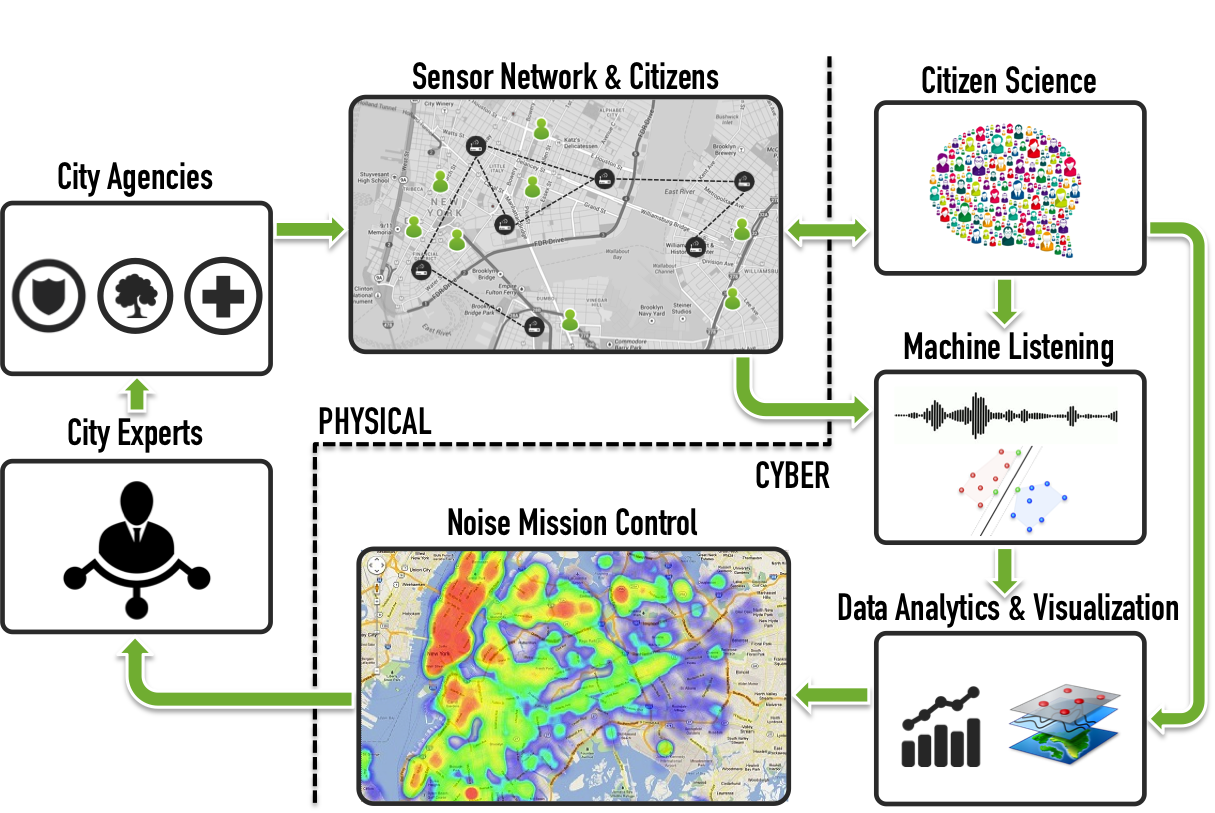
\includegraphics[scale=0.4]{figures/sonyc.png}
                \caption{SONYC project overview (image taken from the project \myhref{https://wp.nyu.edu/sonyc}{website})}
            \end{figure}
        \end{center}
    \end{frame}
    
    \begin{frame}{Introduction: case study}
        
        {\bf Sounds of New York City (SONYC) - } Prototype
        \vfill 
        \begin{center} 
            \begin{figure}
                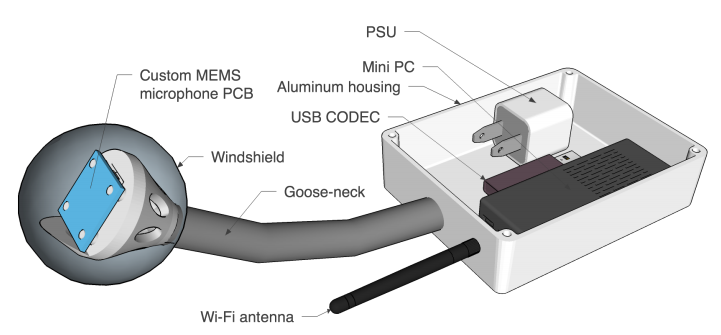
\includegraphics[scale=0.5]{figures/sonyc_prototype}
                \caption{SONYC sensor unit prototype (image taken from the project \myhref{https://wp.nyu.edu/sonyc}{website})}
            \end{figure}
        \end{center}
    \end{frame}
    
\section{Technology background}

    \begin{frame}{Technology background}
        
        {\bf LoRaWAN -} a type of wireless telecommunication that:
        
        \begin{itemize}
            \item allows long range communication
            \item has limited bit rate (amount of information that can be transmitted per packet)
            \item transmitting and receiving data drains very little current from power source
        \end{itemize}
        \begin{center} 
            \begin{figure}
                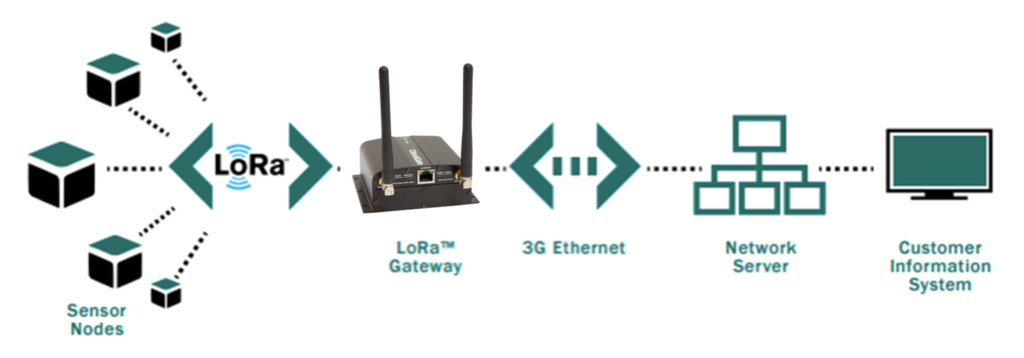
\includegraphics[scale=0.5]{figures/lorawan.png}
                \caption{A typical LoRaWAN based application}
            \end{figure}
        \end{center}
        
    \end{frame}
    
    \begin{frame}{Technology background}
        
        {\bf As a consequence of the LoRaWAN properties -}
        \vfill 
        Sensor node features:
        \begin{itemize}
            \item battery operated 
            \item easy to deploy
            \item low maintenance
            \item pervasive deployment
            \item low cost
            \item discrete
            \item secure
        \end{itemize}
        \vfill 
        Application features:
        \begin{itemize}
            \item low data throughput 
            \item delay tolerant
            \item periodic sensing and/or event based notifications
        \end{itemize}
        
    \end{frame}

\section{Project goals}

    \begin{frame}{Project goals}
    
        {\bf Business goals -} (i) investigate how acoustic sensing can be used to improve the quality of life for Calgarians, (ii) create a platform to test other LoRaWAN-based applications
        \vfill 
        {\bf Research goals -} investigate the limits of LoRaWAN-based applications by incorporating \alert{in-network processing}
        \vfill
        \begin{center}
            \begin{figure}
                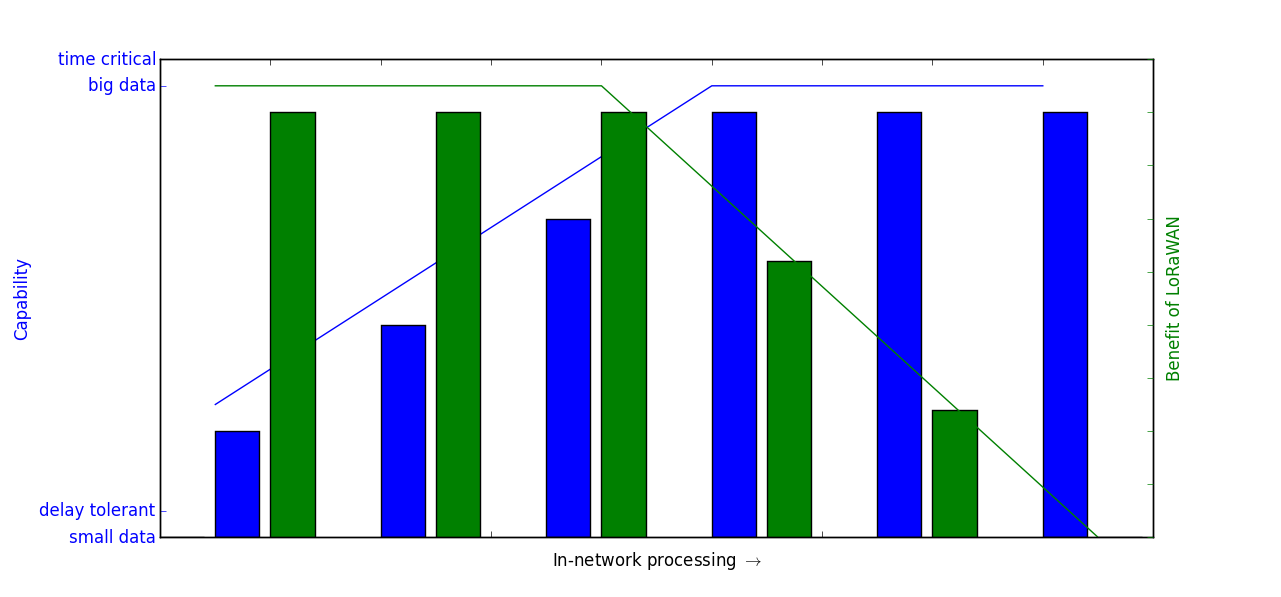
\includegraphics[scale=0.31]{figures/figure_1.png}
            \end{figure}
        \end{center}
        
    \end{frame}

\section{Current project status}

    \begin{frame}{Current project status}
        
        We expect a working prototype by the end of the year.
        \vfill 
        {\bf Microphone specs:} tolerance limits of $\pm 1$dB, noise floor of 30dB (\alert{exceeds} the specifications of a Class 2 sound level meter)
        \vfill
        {\bf Microcontroller:} best possible computing power for the price and power consumption 
        \vfill 
        {\bf Algorithm:} Spectral decomposition. Future implementation: sound source classification. 
        \vfill 
        {\bf Battery life:} 2 months with 2 D-cell Lithium Ion batteries
        \vfill 
        {\bf Physical dimensions:} 8x8x4cm (enclosure only)
        \vfill
        {\bf Price per unit:} \$150
        
    \end{frame}
    
    \begin{frame}{Current project status}
        
        \begin{itemize}
            \item Gateways and network server provided by Tektelic
            \item Application server is developed
        \end{itemize}
        \vfill 
        \begin{center}
            \begin{figure}
                \centering
                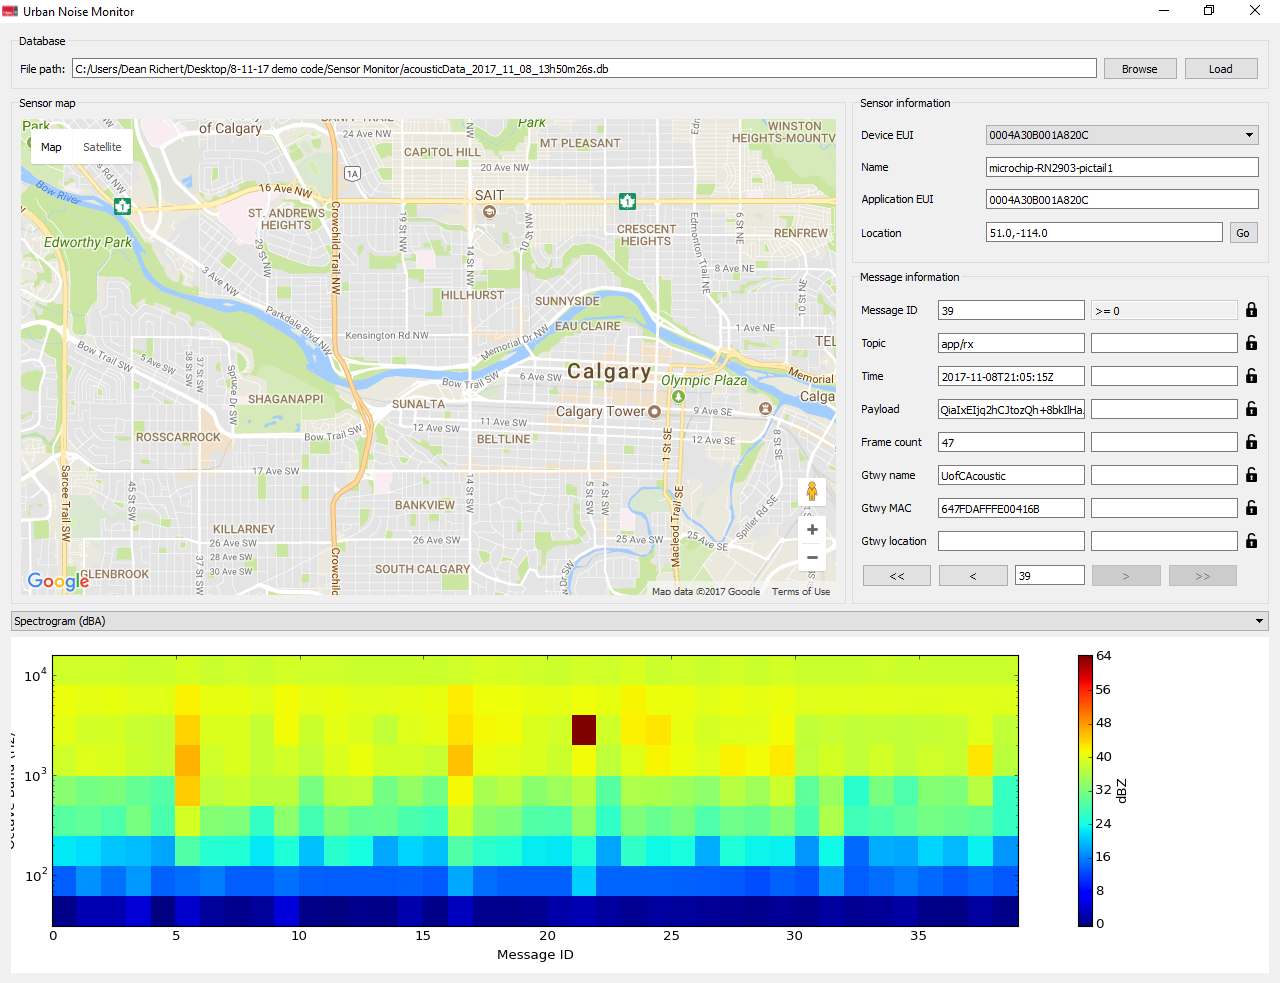
\includegraphics[scale=0.25]{figures/gui.PNG}
            \end{figure}
        \end{center}
        
    \end{frame}


\section{Acoustic sensing basics}

    \begin{frame}{Acoustic sensing basics}
        
        \begin{center}
            \begin{figure}
                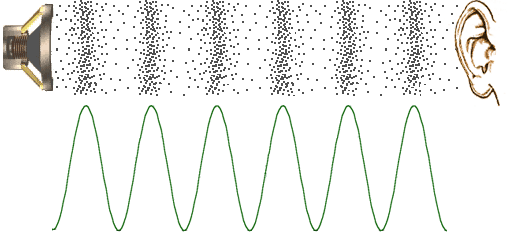
\includegraphics[scale=0.25]{figures/sound_pressure_wave.png}
            \end{figure}
        \end{center}
        
        \begin{itemize}
            \item Sound is an oscillating pressure wave - a microphone is basically a pressure sensor
            \item A decibel reading (dB) is a measure of the power of the sound pressure wave in a window of time
            \item dBA is another common noise level unit that models the perceived loudness of a sound source by humans 
        \end{itemize} 
        
    \end{frame}
    
    \begin{frame}{Acoustic sensing basics}
        
        A typical CoC bylaw reads:
        \begin{center} \fbox{\begin{minipage}{0.75\linewidth}
            \emph{No person shall cause continuous sound that exceeds 75dBA during the day-time (60dBA during the night-time)}
        \end{minipage}}
        \end{center}
        \begin{itemize}
            \item Continuous sound = continuous duration over a 3 minute period, or sporadically for a total of 3 minutes over a 15 minute period. 
            \item Sound level must exceed 5dBA over ambient before it becomes an offence
        \end{itemize}
        For enforcement purposes, a class 2 sound level meter must be used.
        
    \end{frame}

    \begin{frame}{Acoustic sensing basics}
        
        The classification of a sound level meter is governed by the IEC 61672-1:2002 standard.
        \vfill
        The standard defines (i) specifications of the device, (ii) tests to verify conformance, and (iii) a schedule for periodic testing of the device.
        \vfill 
        Disclaimer: I have not read the standard!
        \vfill
        Class 2 devices have tolerance limits of $\pm 1.4$dB and measurement ranges from 35dBA-130dBA
        
    \end{frame}
    
    \begin{frame}{Acoustic sensing basics}
        
        How ``far away" can a sensor measure a sound source?
        \vfill 
        A sensor {\bf does not} measure sound at a distance. It measures air pressure {\bf at the sensor location}.
        \vfill 
        Two concepts are relevant:
        \begin{enumerate}
            \item sound {\bf propagation} - sound is attenuated further from the source
            \item {\bf noise floor} - the minimum sound level that can be measured by a sensor (\alert{independent} of the distance to the sound source).
        \end{enumerate}
        \vfill 
        Example 1: A 100dB noise source could be detected by a sensor with a 35dB noise floor 500m away.   
        \vfill 
        Example 2: A 60dB noise source can be detected by the same sensor at most 5m away. 
    \end{frame}

\section{Questions/feedback}

    \begin{frame}{Questions/feedback}
        \begin{center}
            
\includegraphics[scale=0.2]{figures/36601.png}
        \end{center}
    \end{frame}

\end{document}